\documentclass[9pt,twoside,lineno]{pnas-new}
% Compile in the existing PNAS Overleaf project with its support files.
\templatetype{pnassupportinginfo}

\usepackage{graphicx}
\usepackage{amsmath}
\usepackage{placeins}

\title{Model-based inference of reward identity in the lateral orbitofrontal cortex}
\author{Qingfang Liu, Yao Zhao, Taaseen Khan, Nicole Moussa, Geoffrey Schoenbaum, and Thorsten Kahnt}
\correspondingauthor{Thorsten Kahnt.\\E-mail: thorsten.kahnt@nih.gov}

\renewcommand{\thefigure}{S\arabic{figure}}

\begin{document}
\maketitle
\SItext

\subsection*{Supplementary Methods}

\paragraph*{Behavioral data analysis}

Preconditioning and conditioning performance were quantified as the proportion of correct responses within each run. For comparisons among preconditioning cue-pair types, accuracy from the final Day 2 refresher run was calculated separately for each cue pair and then averaged across the two stimulus sets with equal weighting. Conditioning accuracy was compared among the three outcome-associated cue types in the final conditioning run, pooling across stimulus sets. Differences among cue-pair or cue types were assessed using Friedman tests.

Unanswered trials were counted as incorrect when calculating run-wise learning accuracy. For the final-run conditioning comparison among cue types, trials with missing response times were excluded.

For each probe phase, choice proportions were calculated separately for each participant and pairwise cue comparison, pooling valid trials across runs and stimulus sets. Proportions represented selection of the cue named first in each comparison, irrespective of its presentation position. Trials with missing choices or response times were excluded. Changes in choice proportions and odor pleasantness were calculated as post-meal minus pre-meal values. Changes were tested against zero using two-sided Wilcoxon signed-rank tests, with an uncorrected significance threshold of $p < 0.05$.

\paragraph*{Self-reported hunger and satiety}

Participants also rated hunger and satiety before and after the meal by responding to three questions: “How would you rate your current level of hunger?”, “How would you rate your current level of satiety (feeling full)?”, and “How would you rate your current desire to eat?”. Ratings were made using the same horizontal slider scale as the odor pleasantness ratings.

\paragraph*{Recognition memory task.}

During the recognition memory task, participants judged whether specific character--place pairs had been encountered during preconditioning. Each trial consisted of a 3\,s presentation of the first cue (cue\,1), followed by a 0.3\,s blank interval and a 3\,s presentation of the second cue (cue\,2). Participants then indicated whether the pair was ``old'' or a recombined foil. No corrective feedback was provided. Trials were separated by a jittered 3--8\,s inter-trial interval. The task comprised 36 trials in total (6 cue pairs $\times$ old/foil $\times$ 3 repetitions). Foil pairs were constructed by randomly pairing each first cue (A1, A2 or C) with a second cue (B1, B2 or D) that had not been associated with it during pre-conditioning.

\subsection*{Supplementary Results}

\paragraph*{Self-reported hunger and satiety.}

Ratings showed the expected shifts in hunger, satiety, and desire to eat after the meal ($n = 30$; Fig.~\ref{fig_hunger}). Mean hunger ratings decreased from 1.40 before the meal to $-2.77$ afterward. Mean satiety ratings increased from $-1.40$ to 1.88, and mean desire-to-eat ratings decreased from 1.58 to $-2.43$. All three changes were significant (two-sided Wilcoxon signed-rank tests, all $p < 0.001$, uncorrected). Analyses applied the main-figure participant exclusions, and additionally omitted one participant with missing ratings.

\paragraph*{Recognition memory.}

Recognition accuracy did not differ significantly across the three cue-pair types ($n = 31$; Friedman test: $\chi^2(2) = 1.60$, $p = 0.449$; Fig.~\ref{fig_recog}). Analyses used the main-figure participant exclusions.

\paragraph*{Choice preference and odor pleasantness.}

We examined the relationship between probe choices and odor pleasantness in participants with complete pleasantness data after applying the main-figure exclusions ($n = 30$). Meal-related changes in choice proportions were positively correlated with relative changes in outcome pleasantness for A2$>$A1 ($r = 0.43$, $p = 0.018$), B2$>$B1 ($r = 0.41$, $p = 0.023$), and B2$>$D ($r = 0.42$, $p = 0.019$; Fig.~\ref{fig_probe_change_corr}). Correlations for the remaining three comparisons were positive but nonsignificant (all $p \geq 0.096$).

Choice proportions were also positively correlated with the pleasantness difference between the associated outcomes for all six comparisons, both before the meal ($r = 0.43$--$0.77$, all $p \leq 0.018$) and after the meal ($r = 0.42$--$0.81$, all $p \leq 0.020$; Fig.~\ref{fig_probe_corr_pre_post}). All choice--pleasantness tests were two-sided Pearson correlations, uncorrected for multiple comparisons.

% Supplementary figures, one per page.

\clearpage
\begin{figure}[p]
    \centering
    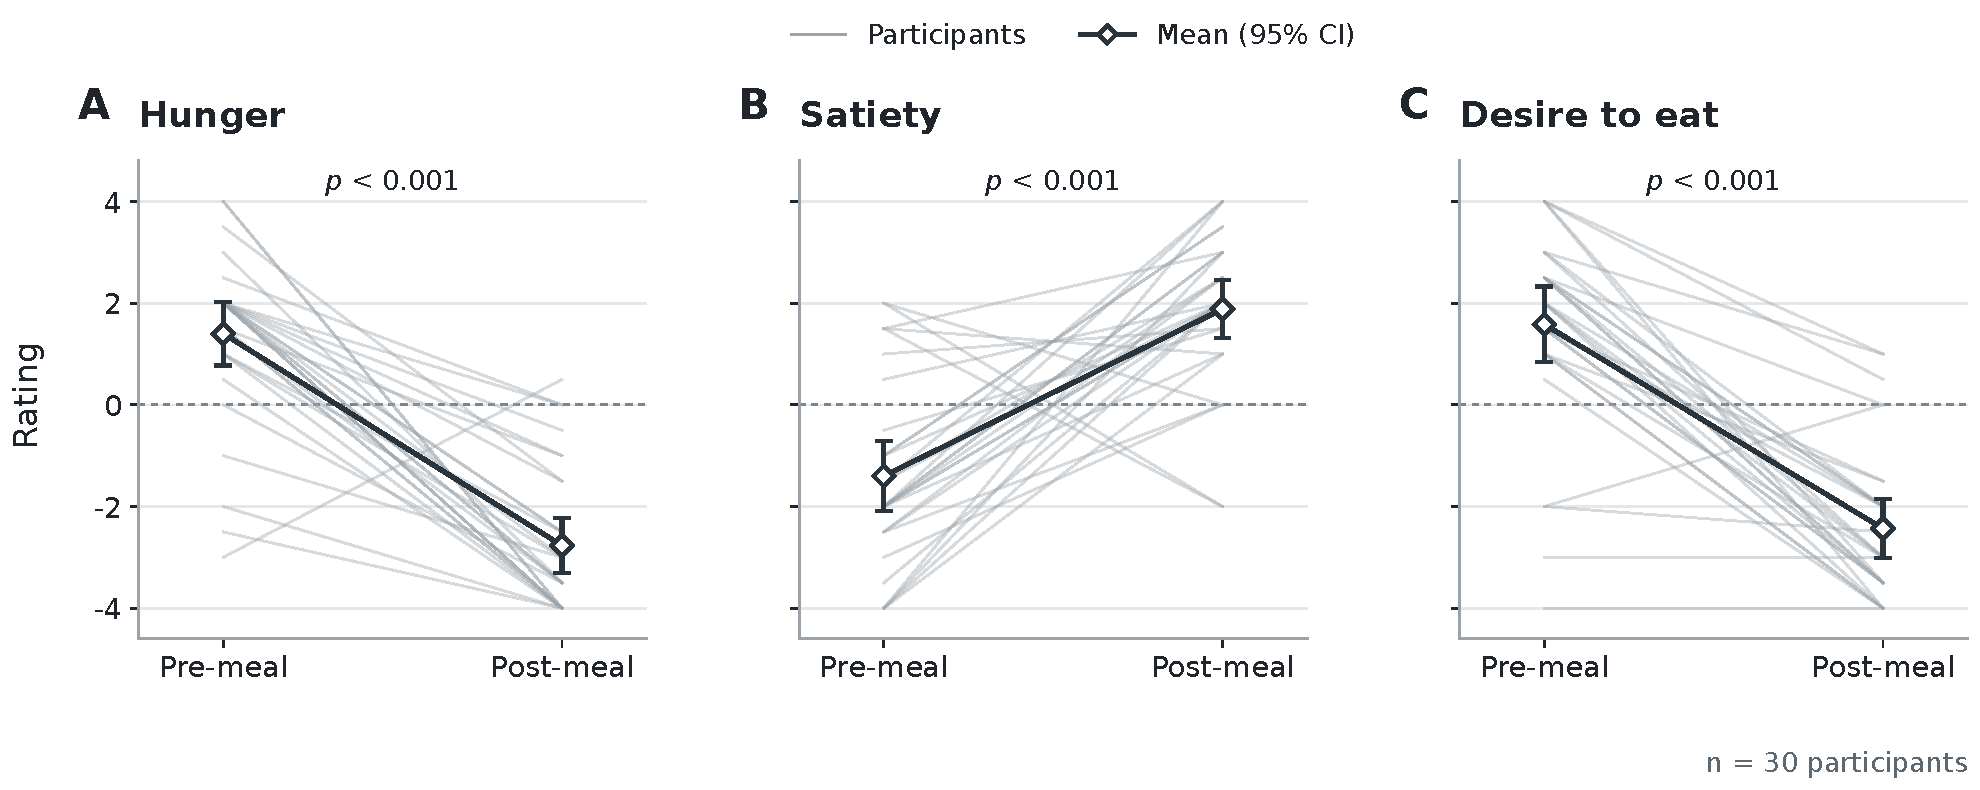
\includegraphics[width=\textwidth]{../../supp_fig/hungry_ratings.pdf}
    \caption{\textbf{Change in self-reported hunger, satiety, and desire to eat.}
Panels A--C show hunger, satiety, and desire-to-eat ratings, respectively, before and after the meal. Gray lines connect measurements from individual participants ($n = 30$). Open diamonds indicate group means, with t-based 95\% confidence intervals. Horizontal dashed lines mark zero on the rating scale. Hunger and desire-to-eat ratings decreased, whereas satiety ratings increased (two-sided Wilcoxon signed-rank tests, all $p < 0.001$, uncorrected for multiple comparisons).}
    \label{fig_hunger}
\end{figure}

\clearpage
\begin{figure}[p]
\centering
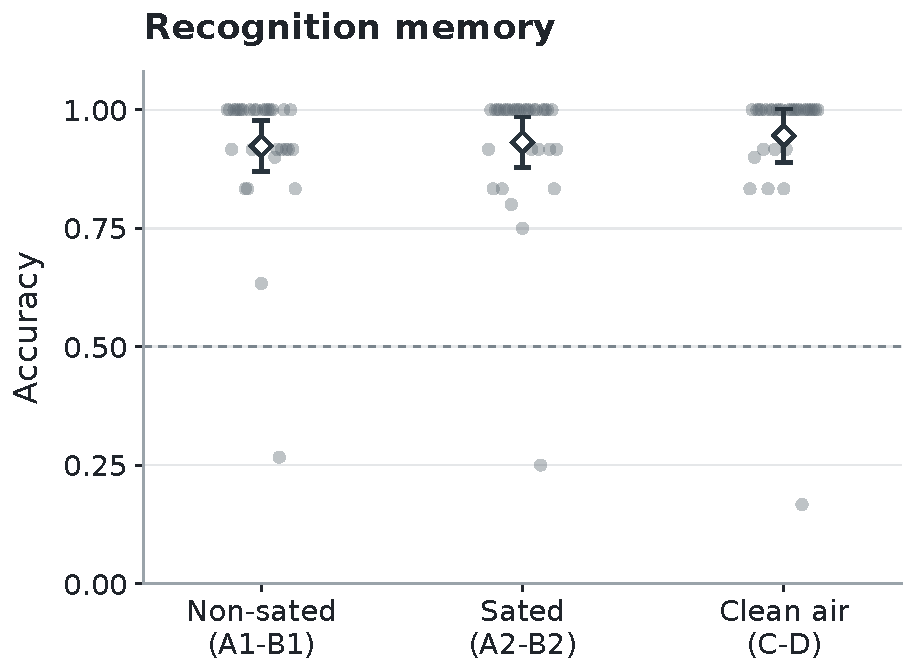
\includegraphics[width=0.48\linewidth]{../../supp_fig/recognition_accuracy.pdf}
\caption{\textbf{Recognition memory accuracy across cue-pair types.}
Points show individual participants' mean recognition accuracy for each cue-pair group ($n = 31$). Accuracy was averaged within each cue pair and then equally across the two pairs in each group. Open diamonds indicate group means, with t-based 95\% confidence intervals. The horizontal dashed line marks chance-level performance (0.5). Recognition accuracy did not differ significantly across cue-pair types (Friedman test: $\chi^2(2) = 1.60$, $p = 0.449$).}
\label{fig_recog}
\end{figure}

\clearpage
\begin{figure}[p]
\centering
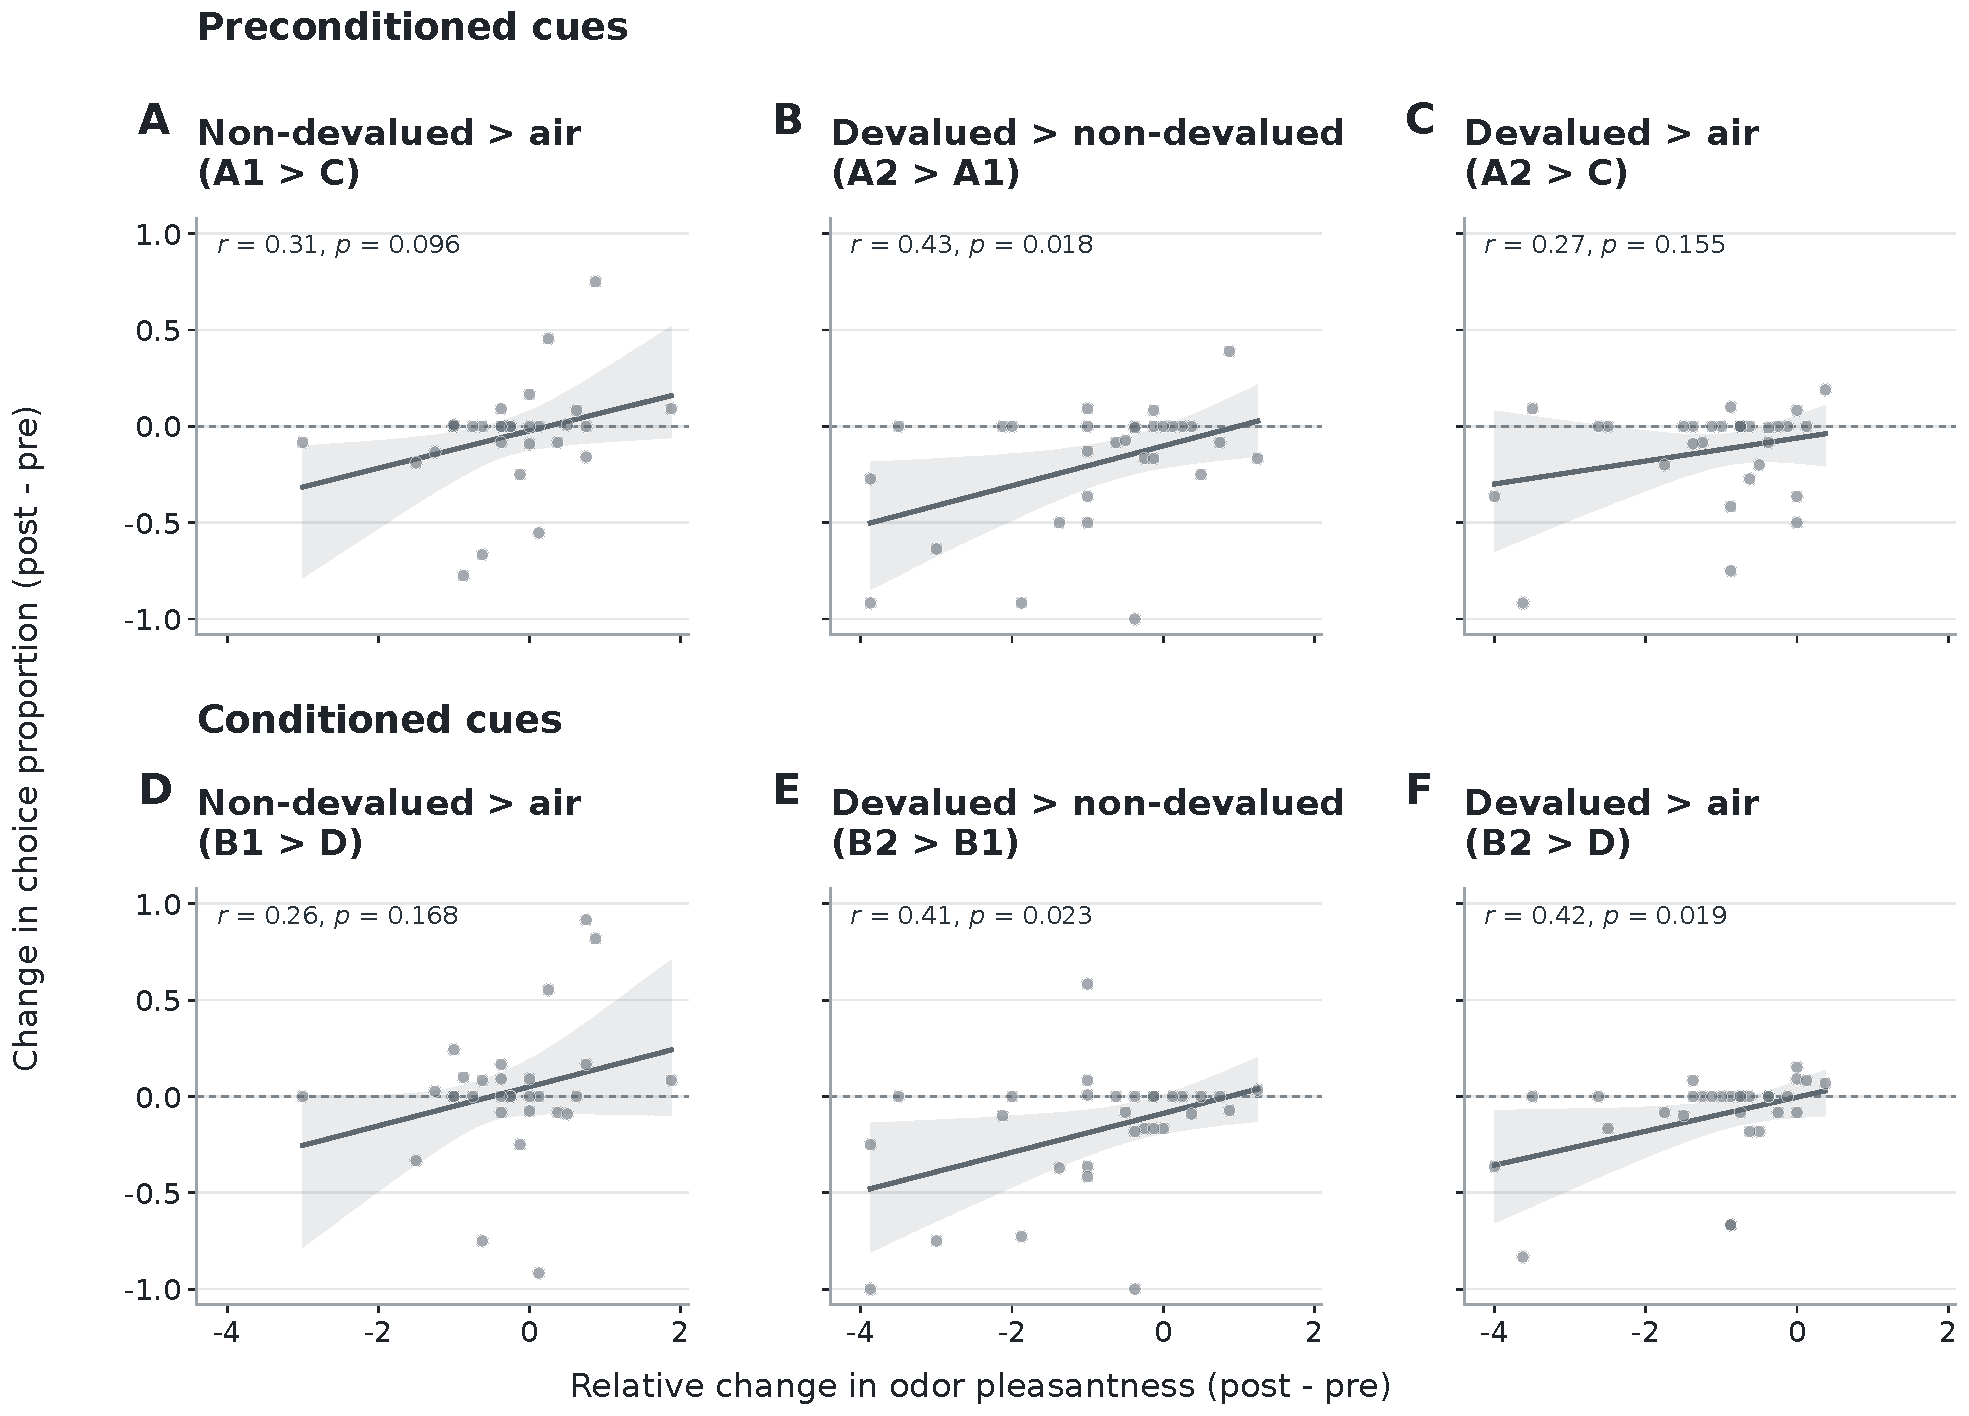
\includegraphics[width=\linewidth]{../../supp_fig/probe_change_corr.pdf}
\caption{\textbf{Changes in choice preference correlate with relative changes in odor pleasantness.}
Panels A--C show preconditioned cues, and panels D--F show conditioned cues. Each point represents one participant ($n = 30$). Choice changes were calculated as post-meal minus pre-meal proportions of choosing the first cue in each comparison. Relative pleasantness change was calculated as the difference between the associated outcomes' post-minus-pre changes in pleasantness ratings, ordered as first cue minus second cue. Lines show ordinary least-squares fits; shaded regions indicate pointwise 95\% bootstrap confidence intervals for the fitted mean. Horizontal dashed lines indicate zero choice change. Positive correlations were significant for A2$>$A1 ($r = 0.43$, $p = 0.018$), B2$>$B1 ($r = 0.41$, $p = 0.023$), and B2$>$D ($r = 0.42$, $p = 0.019$). Correlations were positive but nonsignificant for A1$>$C ($r = 0.31$, $p = 0.096$), A2$>$C ($r = 0.27$, $p = 0.155$), and B1$>$D ($r = 0.26$, $p = 0.168$). All tests were two-sided Pearson correlations, uncorrected for multiple comparisons.}
\label{fig_probe_change_corr}
\end{figure}

\clearpage
\begin{figure}[p]
\centering
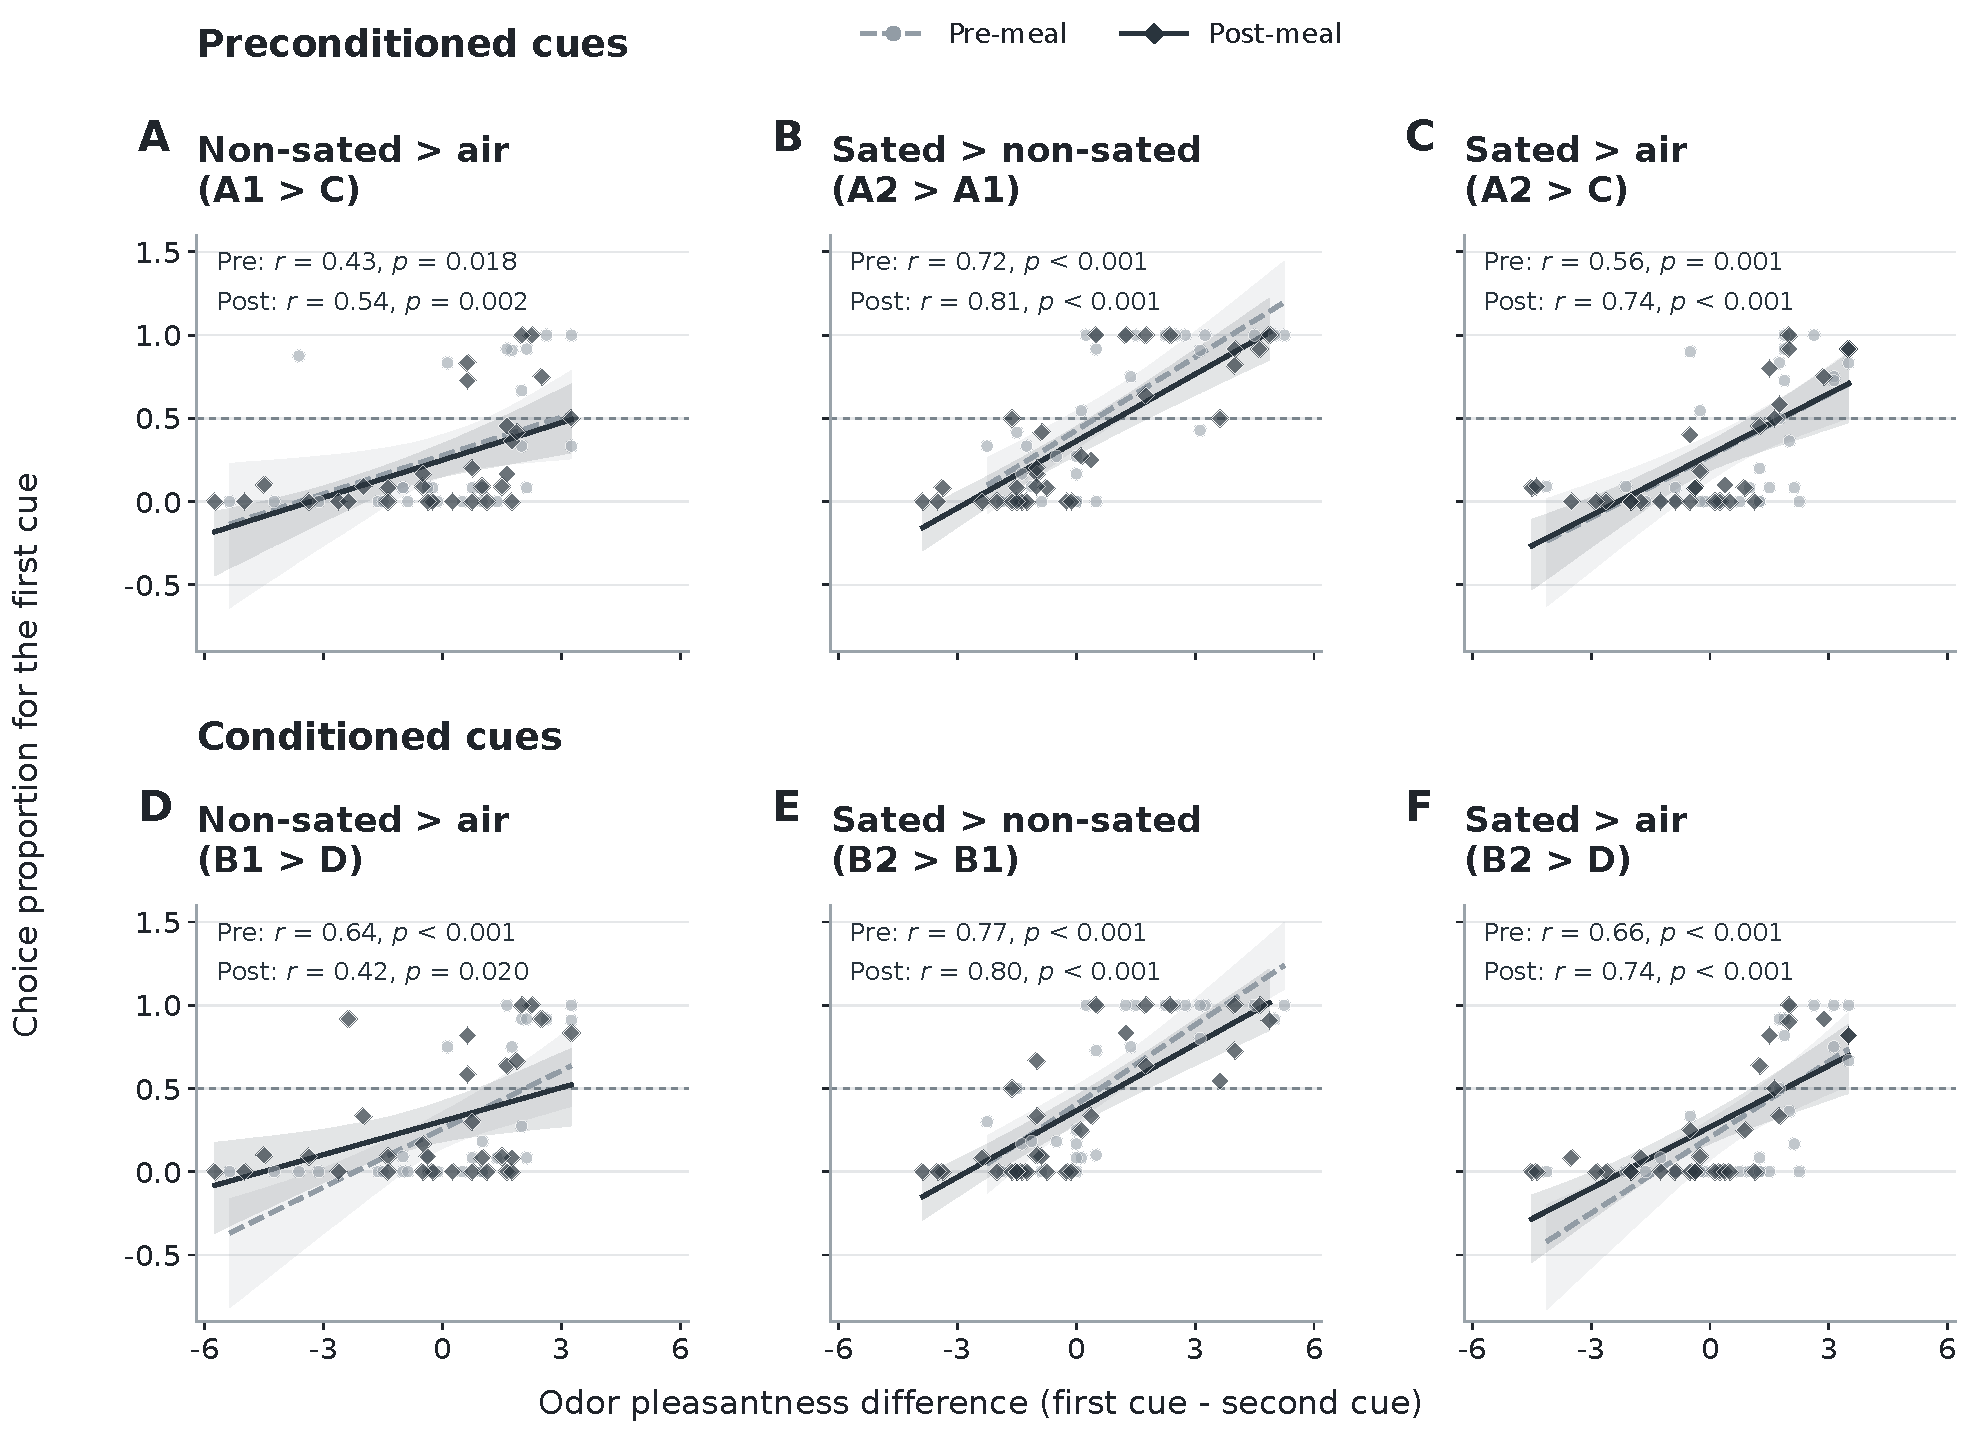
\includegraphics[width=1\linewidth]{../../supp_fig/probe_corr_pre_post.pdf}
\caption{\textbf{Choice preference correlates with odor pleasantness before and after the meal.}
Panels A--C show preconditioned cues, and panels D--F show conditioned cues. Each point represents one participant ($n = 30$). Choice proportions for the first cue in each comparison are plotted against the pleasantness difference between the associated outcomes, ordered as first cue minus second cue. Light-gray circles and dashed regression lines represent pre-meal measurements; dark diamonds and solid regression lines represent post-meal measurements. Lines show ordinary least-squares fits; shaded regions indicate pointwise 95\% bootstrap confidence intervals for the fitted mean. Horizontal dashed lines indicate chance choice (0.5). Positive correlations were significant in both phases for all six comparisons: A1$>$C (pre: $r = 0.43$, $p = 0.018$; post: $r = 0.54$, $p = 0.002$), A2$>$A1 (pre: $r = 0.72$, $p < 0.001$; post: $r = 0.81$, $p < 0.001$), A2$>$C (pre: $r = 0.56$, $p = 0.001$; post: $r = 0.74$, $p < 0.001$), B1$>$D (pre: $r = 0.64$, $p < 0.001$; post: $r = 0.42$, $p = 0.020$), B2$>$B1 (pre: $r = 0.77$, $p < 0.001$; post: $r = 0.80$, $p < 0.001$), and B2$>$D (pre: $r = 0.66$, $p < 0.001$; post: $r = 0.74$, $p < 0.001$). All tests were two-sided Pearson correlations, uncorrected for multiple comparisons.}
\label{fig_probe_corr_pre_post}
\end{figure}

\FloatBarrier

\end{document}
